\documentclass[8pt,aspectratio=169]{beamer}
\usetheme{Madrid}
\usepackage{graphicx}
\usepackage{booktabs}
\usepackage{adjustbox}
\usepackage{multicol}
\usepackage{amsmath}
\usepackage{amssymb}
\usepackage{listings}
\usepackage{xcolor}

% Color definitions
\definecolor{mlblue}{RGB}{0,102,204}
\definecolor{mlpurple}{RGB}{51,51,178}
\definecolor{mllavender}{RGB}{173,173,224}
\definecolor{mllavender2}{RGB}{193,193,232}
\definecolor{mllavender3}{RGB}{204,204,235}
\definecolor{mllavender4}{RGB}{214,214,239}
\definecolor{mlorange}{RGB}{255, 127, 14}
\definecolor{mlgreen}{RGB}{44, 160, 44}
\definecolor{mlred}{RGB}{214, 39, 40}
\definecolor{mlgray}{RGB}{127, 127, 127}

% Additional colors for template compatibility
\definecolor{lightgray}{RGB}{240, 240, 240}
\definecolor{midgray}{RGB}{180, 180, 180}

% Solidity colors
\definecolor{solkeyword}{RGB}{0,102,153}
\definecolor{solstring}{RGB}{163,21,21}
\definecolor{solcomment}{RGB}{0,128,0}
\definecolor{solnumber}{RGB}{0,128,128}

% Solidity language definition
\lstdefinelanguage{Solidity}{
  keywords={pragma, solidity, contract, function, public, private, external, internal, view, pure, payable, returns, return, if, else, for, while, mapping, address, uint, uint256, int, string, bool, bytes, bytes32, event, emit, modifier, require, constructor, memory, storage, calldata, msg, sender, value, this, new, delete, true, false},
  keywordstyle=\color{solkeyword}\bfseries,
  sensitive=true,
  comment=[l]{//},
  morecomment=[s]{/*}{*/},
  commentstyle=\color{solcomment}\ttfamily,
  stringstyle=\color{solstring}\ttfamily,
  morestring=[b]',
  morestring=[b]"
}

% Apply custom colors to Madrid theme
\setbeamercolor{palette primary}{bg=mllavender3,fg=mlpurple}
\setbeamercolor{palette secondary}{bg=mllavender2,fg=mlpurple}
\setbeamercolor{palette tertiary}{bg=mllavender,fg=white}
\setbeamercolor{palette quaternary}{bg=mlpurple,fg=white}
\setbeamercolor{structure}{fg=mlpurple}
\setbeamercolor{section in toc}{fg=mlpurple}
\setbeamercolor{subsection in toc}{fg=mlblue}
\setbeamercolor{title}{fg=mlpurple}
\setbeamercolor{frametitle}{fg=mlpurple,bg=mllavender3}
\setbeamercolor{block title}{bg=mllavender2,fg=mlpurple}
\setbeamercolor{block body}{bg=mllavender4,fg=black}

\setbeamertemplate{navigation symbols}{}
\setbeamertemplate{itemize items}[circle]
\setbeamertemplate{enumerate items}[default]
\setbeamersize{text margin left=5mm,text margin right=5mm}

\newcommand{\bottomnote}[1]{%
\vfill
\vspace{-2mm}
\textcolor{mllavender2}{\rule{\textwidth}{0.4pt}}
\vspace{1mm}
\footnotesize
\textbf{#1}
}

% TikZ and pgfplots packages
\usepackage{tikz}
\usepackage{pgfplots}
\pgfplotsset{compat=1.18}
\usetikzlibrary{arrows.meta, positioning, shapes.geometric, shapes.symbols, calc, decorations.pathmorphing, mindmap}

\title{NFTs \& Digital Assets: A Visual Introduction}
\subtitle{Standalone Mini-Lecture}
\author{Prof.~Dr.~Joerg Osterrieder}
\institute{University Lecture Series}
\date{\today}
\begin{document}

% ==================== FRAME 1: TITLE ====================
\begin{frame}[plain]
\vspace{2cm}
\begin{center}
{\Huge\color{mlpurple} NFTs \& Digital Assets: A Visual Introduction}\\[0.4cm]
{\Large\color{mlblue} Standalone Mini-Lecture}\\[0.3cm]
\textcolor{mlgray}{\rule{6cm}{0.4pt}}\\[0.3cm]
{\small\itshape ``Own the original --- in a world of infinite copies''}\\[1.5cm]
{\normalsize Prof.~Dr.~Joerg Osterrieder}\\[0.2cm]
{\small University Lecture Series}\\[0.2cm]
{\small \today}
\end{center}
\end{frame}

% ==================== FRAME 2: THE DIGITAL OWNERSHIP PROBLEM ====================
\begin{frame}{The Digital Ownership Problem}
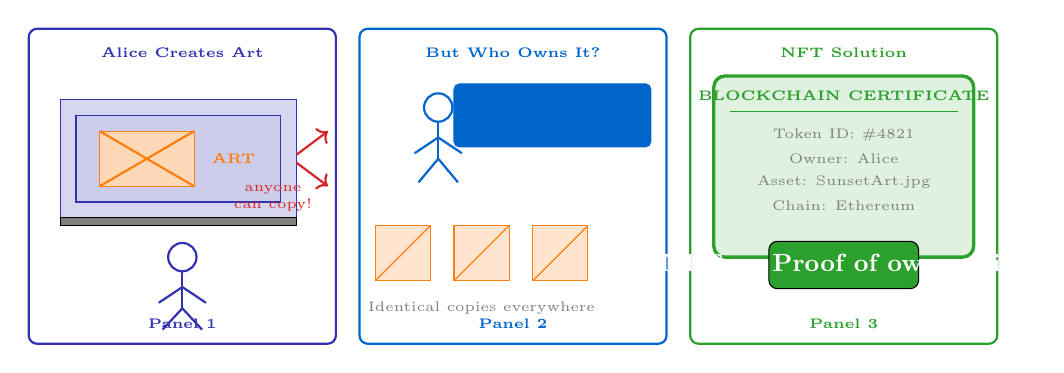
\begin{tikzpicture}
  % Panel borders
  \draw[thick, mlpurple, rounded corners=3pt] (0.1,0.2) rectangle (4.0,4.2);
  \draw[thick, mlblue,   rounded corners=3pt] (4.3,0.2) rectangle (8.2,4.2);
  \draw[thick, mlgreen,  rounded corners=3pt] (8.5,0.2) rectangle (12.4,4.2);

  % --- Panel 1: Alice creates art, anyone can copy ---
  \node[font=\tiny\bfseries, mlpurple] at (2.05,3.9) {Alice Creates Art};
  % Laptop
  \draw[fill=mllavender4, draw=mlpurple] (0.5,1.8) rectangle (3.5,3.3);
  \draw[fill=mllavender3, draw=mlpurple] (0.7,2.0) rectangle (3.3,3.1);
  % Art picture on screen
  \draw[fill=mlorange!30, draw=mlorange] (1.0,2.2) rectangle (2.2,2.9);
  \draw[mlorange, thick] (1.0,2.2) -- (2.2,2.9);
  \draw[mlorange, thick] (1.0,2.9) -- (2.2,2.2);
  \node[font=\tiny\bfseries, mlorange] at (2.7,2.55) {ART};
  \draw[fill=mlgray] (0.5,1.7) rectangle (3.5,1.8);
  % Alice stick figure
  \draw[mlpurple,thick] (2.05,1.3) circle (0.18);
  \draw[mlpurple,thick] (2.05,1.12) -- (2.05,0.65);
  \draw[mlpurple,thick] (2.05,0.92) -- (1.75,0.72);
  \draw[mlpurple,thick] (2.05,0.92) -- (2.35,0.72);
  \draw[mlpurple,thick] (2.05,0.65) -- (1.80,0.38);
  \draw[mlpurple,thick] (2.05,0.65) -- (2.30,0.38);
  % Copy arrows
  \draw[->, mlred, thick] (3.5,2.6) -- (3.9,2.9);
  \draw[->, mlred, thick] (3.5,2.5) -- (3.9,2.2);
  \node[font=\tiny, mlred, align=center] at (3.2,2.05) {anyone\\can copy!};
  \node[font=\tiny\bfseries, mlpurple] at (2.05,0.45) {Panel 1};

  % --- Panel 2: Bob asks how to prove ownership ---
  \node[font=\tiny\bfseries, mlblue] at (6.25,3.9) {But Who Owns It?};
  % Bob stick figure
  \draw[mlblue,thick] (5.3,3.2) circle (0.18);
  \draw[mlblue,thick] (5.3,3.02) -- (5.3,2.55);
  \draw[mlblue,thick] (5.3,2.82) -- (5.0,2.62);
  \draw[mlblue,thick] (5.3,2.82) -- (5.6,2.62);
  \draw[mlblue,thick] (5.3,2.55) -- (5.05,2.25);
  \draw[mlblue,thick] (5.3,2.55) -- (5.55,2.25);
  % Speech bubble from Bob
  \draw[fill=white, mlblue, rounded corners=2pt] (5.5,2.7) rectangle (8.0,3.5);
  \node[font=\tiny, mlblue, align=center] at (6.75,3.1) {How do you prove\\you own it?\\Anyone has a copy!};
  % Multiple identical copies
  \draw[fill=mlorange!20, draw=mlorange] (4.5,1.0) rectangle (5.2,1.7);
  \draw[mlorange, thin] (4.5,1.0) -- (5.2,1.7);
  \draw[fill=mlorange!20, draw=mlorange] (5.5,1.0) rectangle (6.2,1.7);
  \draw[mlorange, thin] (5.5,1.0) -- (6.2,1.7);
  \draw[fill=mlorange!20, draw=mlorange] (6.5,1.0) rectangle (7.2,1.7);
  \draw[mlorange, thin] (6.5,1.0) -- (7.2,1.7);
  \node[font=\tiny, mlgray, align=center] at (5.85,0.65) {Identical copies everywhere};
  \node[font=\tiny\bfseries, mlblue] at (6.25,0.45) {Panel 2};

  % --- Panel 3: NFT certificate with checkmark ---
  \node[font=\tiny\bfseries, mlgreen] at (10.45,3.9) {NFT Solution};
  % Certificate/document
  \draw[fill=mlgreen!15, draw=mlgreen, very thick, rounded corners=4pt]
       (8.8,1.3) rectangle (12.1,3.6);
  \node[font=\tiny\bfseries, mlgreen] at (10.45,3.35) {BLOCKCHAIN CERTIFICATE};
  \draw[mlgreen, thin] (9.0,3.15) -- (11.9,3.15);
  \node[font=\tiny, mlgray, align=center] at (10.45,2.85) {Token ID: \#4821};
  \node[font=\tiny, mlgray, align=center] at (10.45,2.55) {Owner: Alice};
  \node[font=\tiny, mlgray, align=center] at (10.45,2.25) {Asset: SunsetArt.jpg};
  \node[font=\tiny, mlgray, align=center] at (10.45,1.95) {Chain: Ethereum};
  % Checkmark badge
  \draw[fill=mlgreen, rounded corners=3pt] (9.5,0.9) rectangle (11.4,1.5);
  \node[font=\small\bfseries, white, align=center] at (10.45,1.2) {NFT --- Proof of ownership!};
  \node[font=\tiny\bfseries, mlgreen] at (10.45,0.45) {Panel 3};
\end{tikzpicture}

\bottomnote{NFTs solve the digital ownership problem by creating verifiable scarcity on-chain.}
\end{frame}

% ==================== FRAME 3: WHAT IS AN NFT? ====================
\begin{frame}{What is an NFT?}
\begin{columns}[c]
  \begin{column}{0.44\textwidth}
    \centering
    {\small\bfseries\color{mlblue} Fungible Tokens}\\[0.2cm]
    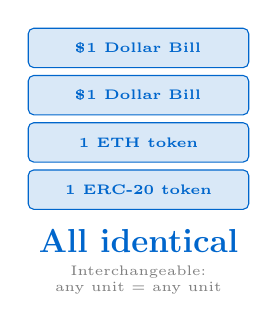
\begin{tikzpicture}
      % Dollar bills -- identical
      \draw[fill=mlblue!15, draw=mlblue, rounded corners=2pt] (0.0,3.4) rectangle (2.8,3.9);
      \node[font=\tiny\bfseries, mlblue] at (1.4,3.65) {\$1 Dollar Bill};
      \draw[fill=mlblue!15, draw=mlblue, rounded corners=2pt] (0.0,2.8) rectangle (2.8,3.3);
      \node[font=\tiny\bfseries, mlblue] at (1.4,3.05) {\$1 Dollar Bill};
      \draw[fill=mlblue!15, draw=mlblue, rounded corners=2pt] (0.0,2.2) rectangle (2.8,2.7);
      \node[font=\tiny\bfseries, mlblue] at (1.4,2.45) {1 ETH token};
      \draw[fill=mlblue!15, draw=mlblue, rounded corners=2pt] (0.0,1.6) rectangle (2.8,2.1);
      \node[font=\tiny\bfseries, mlblue] at (1.4,1.85) {1 ERC-20 token};
      % Equal sign
      \node[font=\large\bfseries, mlblue] at (1.4,1.2) {All identical};
      \node[font=\tiny, mlgray, align=center] at (1.4,0.7) {Interchangeable:\\any unit = any unit};
    \end{tikzpicture}
  \end{column}

  \begin{column}{0.12\textwidth}
    \centering
    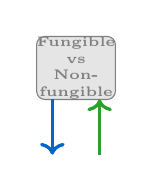
\begin{tikzpicture}
      \draw[fill=mlgray!20, draw=mlgray, rounded corners=3pt]
            (-0.3,1.5) rectangle (0.7,2.3);
      \node[font=\tiny\bfseries, mlgray, align=center] at (0.2,1.9)
            {Fungible\\vs\\Non-\\fungible};
      \draw[->, very thick, mlblue]  (-0.1,1.5) -- (-0.1,0.8);
      \draw[->, very thick, mlgreen]  (0.5,0.8) -- (0.5,1.5);
    \end{tikzpicture}
  \end{column}

  \begin{column}{0.44\textwidth}
    \centering
    {\small\bfseries\color{mlgreen} Non-Fungible Tokens}\\[0.2cm]
    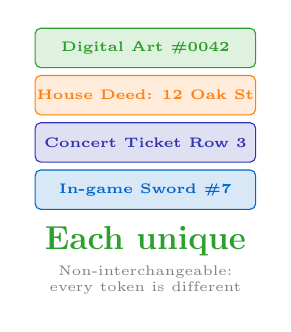
\begin{tikzpicture}
      % Unique items
      \draw[fill=mlgreen!15, draw=mlgreen, rounded corners=2pt] (0.0,3.4) rectangle (2.8,3.9);
      \node[font=\tiny\bfseries, mlgreen] at (1.4,3.65) {Digital Art \#0042};
      \draw[fill=mlorange!15, draw=mlorange, rounded corners=2pt] (0.0,2.8) rectangle (2.8,3.3);
      \node[font=\tiny\bfseries, mlorange] at (1.4,3.05) {House Deed: 12 Oak St};
      \draw[fill=mlpurple!15, draw=mlpurple, rounded corners=2pt] (0.0,2.2) rectangle (2.8,2.7);
      \node[font=\tiny\bfseries, mlpurple] at (1.4,2.45) {Concert Ticket Row 3};
      \draw[fill=mlblue!15, draw=mlblue, rounded corners=2pt] (0.0,1.6) rectangle (2.8,2.1);
      \node[font=\tiny\bfseries, mlblue] at (1.4,1.85) {In-game Sword \#7};
      % Unique label
      \node[font=\large\bfseries, mlgreen] at (1.4,1.2) {Each unique};
      \node[font=\tiny, mlgray, align=center] at (1.4,0.7) {Non-interchangeable:\\every token is different};
    \end{tikzpicture}
  \end{column}
\end{columns}

\bottomnote{Fungible = interchangeable (every dollar is the same). Non-fungible = unique (every NFT is different).}
\end{frame}

% ==================== FRAME 4: HOW NFTs WORK ====================
\begin{frame}{How NFTs Work}
\centering
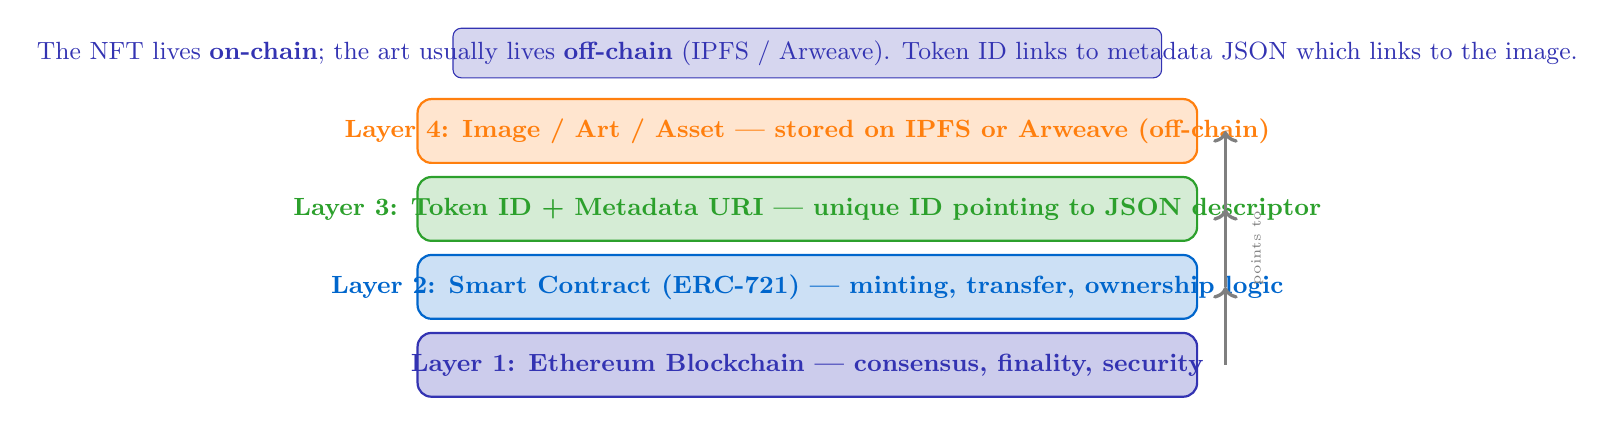
\begin{tikzpicture}[scale=0.90]
  % Layer 1 -- Ethereum blockchain (bottom)
  \draw[fill=mlpurple!25, draw=mlpurple, rounded corners=5pt, thick]
       (0,0) rectangle (11,0.9);
  \node[font=\small\bfseries, mlpurple, align=center] at (5.5,0.45)
       {Layer 1: Ethereum Blockchain --- consensus, finality, security};

  % Layer 2 -- ERC-721 Smart Contract
  \draw[fill=mlblue!20, draw=mlblue, rounded corners=5pt, thick]
       (0,1.1) rectangle (11,2.0);
  \node[font=\small\bfseries, mlblue, align=center] at (5.5,1.55)
       {Layer 2: Smart Contract (ERC-721) --- minting, transfer, ownership logic};

  % Layer 3 -- Token ID + Metadata URI
  \draw[fill=mlgreen!20, draw=mlgreen, rounded corners=5pt, thick]
       (0,2.2) rectangle (11,3.1);
  \node[font=\small\bfseries, mlgreen, align=center] at (5.5,2.65)
       {Layer 3: Token ID + Metadata URI --- unique ID pointing to JSON descriptor};

  % Layer 4 -- Image/Art/Asset (top)
  \draw[fill=mlorange!20, draw=mlorange, rounded corners=5pt, thick]
       (0,3.3) rectangle (11,4.2);
  \node[font=\small\bfseries, mlorange, align=center] at (5.5,3.75)
       {Layer 4: Image / Art / Asset --- stored on IPFS or Arweave (off-chain)};

  % Upward arrows
  \draw[->, very thick, mlgray] (11.4,0.45) -- (11.4,1.55);
  \draw[->, very thick, mlgray] (11.4,1.55) -- (11.4,2.65);
  \draw[->, very thick, mlgray] (11.4,2.65) -- (11.4,3.75);
  \node[font=\tiny, mlgray, rotate=90] at (11.85,2.1) {points to};

  % Side note box
  \draw[fill=mllavender4, draw=mlpurple, rounded corners=3pt]
       (0.5,4.5) rectangle (10.5,5.2);
  \node[font=\small, mlpurple, align=center] at (5.5,4.85)
       {The NFT lives \textbf{on-chain}; the art usually lives \textbf{off-chain} (IPFS / Arweave).
        Token ID links to metadata JSON which links to the image.};
\end{tikzpicture}

\bottomnote{An NFT is a smart contract entry pointing to metadata -- the media itself is usually stored off-chain.}
\end{frame}

% ==================== FRAME 5: NFT MARKETPLACES ====================
\begin{frame}{NFT Marketplaces}
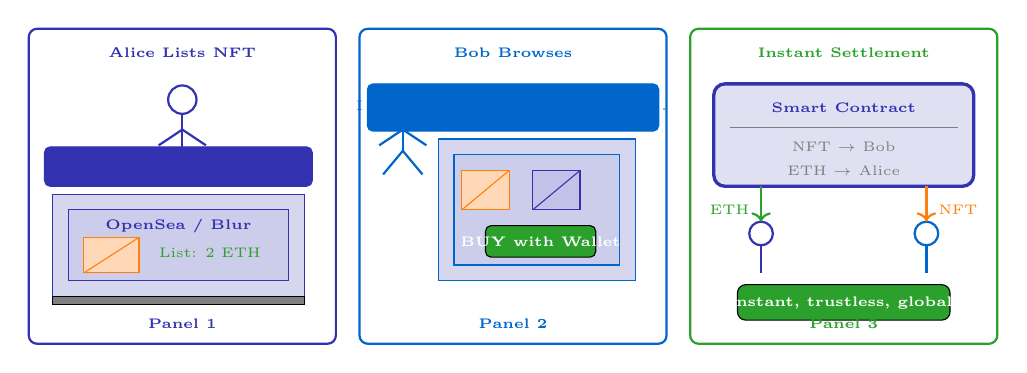
\begin{tikzpicture}
  % Panel borders
  \draw[thick, mlpurple, rounded corners=3pt] (0.1,0.2) rectangle (4.0,4.2);
  \draw[thick, mlblue,   rounded corners=3pt] (4.3,0.2) rectangle (8.2,4.2);
  \draw[thick, mlgreen,  rounded corners=3pt] (8.5,0.2) rectangle (12.4,4.2);

  % --- Panel 1: Alice lists NFT ---
  \node[font=\tiny\bfseries, mlpurple] at (2.05,3.9) {Alice Lists NFT};
  % Alice stick figure
  \draw[mlpurple,thick] (2.05,3.3) circle (0.18);
  \draw[mlpurple,thick] (2.05,3.12) -- (2.05,2.65);
  \draw[mlpurple,thick] (2.05,2.92) -- (1.75,2.72);
  \draw[mlpurple,thick] (2.05,2.92) -- (2.35,2.72);
  \draw[mlpurple,thick] (2.05,2.65) -- (1.80,2.35);
  \draw[mlpurple,thick] (2.05,2.65) -- (2.30,2.35);
  % Marketplace screen
  \draw[fill=mllavender4, draw=mlpurple] (0.4,0.8) rectangle (3.6,2.1);
  \draw[fill=mllavender3, draw=mlpurple] (0.6,1.0) rectangle (3.4,1.9);
  \node[font=\tiny\bfseries, mlpurple] at (2.0,1.7) {OpenSea / Blur};
  \draw[fill=mlorange!30, draw=mlorange] (0.8,1.1) rectangle (1.5,1.55);
  \draw[mlorange, thin] (0.8,1.1) -- (1.5,1.55);
  \node[font=\tiny, mlgreen] at (2.4,1.35) {List: 2 ETH};
  \draw[fill=mlgray] (0.4,0.7) rectangle (3.6,0.8);
  % Speech bubble
  \draw[fill=white, mlpurple, rounded corners=2pt] (0.3,2.2) rectangle (3.7,2.7);
  \node[font=\tiny, mlpurple, align=center] at (2.0,2.45) {I'll list my NFT for 2 ETH!};
  \node[font=\tiny\bfseries, mlpurple] at (2.05,0.45) {Panel 1};

  % --- Panel 2: Bob browses and buys ---
  \node[font=\tiny\bfseries, mlblue] at (6.25,3.9) {Bob Browses};
  % Bob stick figure
  \draw[mlblue,thick] (4.85,3.3) circle (0.18);
  \draw[mlblue,thick] (4.85,3.12) -- (4.85,2.65);
  \draw[mlblue,thick] (4.85,2.92) -- (4.55,2.72);
  \draw[mlblue,thick] (4.85,2.92) -- (5.15,2.72);
  \draw[mlblue,thick] (4.85,2.65) -- (4.60,2.35);
  \draw[mlblue,thick] (4.85,2.65) -- (5.10,2.35);
  % Tablet/phone
  \draw[fill=mllavender4, draw=mlblue] (5.3,1.0) rectangle (7.8,2.8);
  \draw[fill=mllavender3, draw=mlblue] (5.5,1.2) rectangle (7.6,2.6);
  % NFT thumbnails
  \draw[fill=mlorange!30, draw=mlorange] (5.6,1.9) rectangle (6.2,2.4);
  \draw[mlorange, thin] (5.6,1.9) -- (6.2,2.4);
  \draw[fill=mlpurple!30, draw=mlpurple] (6.5,1.9) rectangle (7.1,2.4);
  \draw[mlpurple, thin] (6.5,1.9) -- (7.1,2.4);
  % Buy button
  \draw[fill=mlgreen, rounded corners=2pt] (5.9,1.3) rectangle (7.3,1.7);
  \node[font=\tiny\bfseries, white] at (6.6,1.5) {BUY with Wallet};
  % Speech bubble
  \draw[fill=white, mlblue, rounded corners=2pt] (4.4,2.9) rectangle (8.1,3.5);
  \node[font=\tiny, mlblue, align=center] at (6.25,3.2) {I want this one. Connecting wallet\ldots};
  \node[font=\tiny\bfseries, mlblue] at (6.25,0.45) {Panel 2};

  % --- Panel 3: Smart contract transfers ---
  \node[font=\tiny\bfseries, mlgreen] at (10.45,3.9) {Instant Settlement};
  % Smart contract box
  \draw[fill=mlpurple!15, draw=mlpurple, very thick, rounded corners=4pt]
       (8.8,2.2) rectangle (12.1,3.5);
  \node[font=\tiny\bfseries, mlpurple, align=center] at (10.45,3.2) {Smart Contract};
  \draw[mlgray, thin] (9.0,2.95) -- (11.9,2.95);
  \node[font=\tiny, mlgray, align=center] at (10.45,2.7) {NFT $\rightarrow$ Bob};
  \node[font=\tiny, mlgray, align=center] at (10.45,2.4) {ETH $\rightarrow$ Alice};
  % Alice receives ETH
  \draw[mlpurple,thick] (9.4,1.6) circle (0.15);
  \draw[mlpurple,thick] (9.4,1.45) -- (9.4,1.1);
  \draw[->, thick, mlgreen] (9.4,2.2) -- (9.4,1.75);
  \node[font=\tiny, mlgreen] at (9.0,1.9) {ETH};
  % Bob receives NFT
  \draw[mlblue,thick] (11.5,1.6) circle (0.15);
  \draw[mlblue,thick] (11.5,1.45) -- (11.5,1.1);
  \draw[->, thick, mlorange] (11.5,2.2) -- (11.5,1.75);
  \node[font=\tiny, mlorange] at (11.9,1.9) {NFT};
  % Badge
  \draw[fill=mlgreen, rounded corners=3pt] (9.1,0.5) rectangle (11.8,0.95);
  \node[font=\tiny\bfseries, white, align=center] at (10.45,0.72) {Instant, trustless, global!};
  \node[font=\tiny\bfseries, mlgreen] at (10.45,0.45) {Panel 3};
\end{tikzpicture}

\bottomnote{NFT marketplaces are smart contract platforms -- no middleman holds the assets.}
\end{frame}

% ==================== FRAME 6: MINTING YOUR FIRST NFT ====================
\begin{frame}{Minting Your First NFT}
\centering
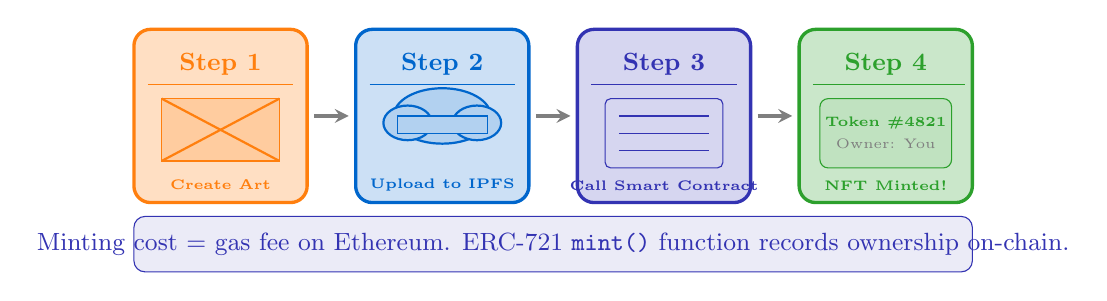
\begin{tikzpicture}[scale=0.88]
  % Step 1 -- Create Art
  \draw[fill=mlorange!25, draw=mlorange, very thick, rounded corners=6pt]
       (0,1.5) rectangle (2.5,4.0);
  \node[font=\small\bfseries, mlorange, align=center] at (1.25,3.5) {Step 1};
  \draw[mlorange, thin] (0.2,3.2) -- (2.3,3.2);
  % Art icon
  \draw[fill=mlorange!40, draw=mlorange] (0.4,2.1) rectangle (2.1,3.0);
  \draw[mlorange, thick] (0.4,2.1) -- (2.1,3.0);
  \draw[mlorange, thick] (0.4,3.0) -- (2.1,2.1);
  \node[font=\tiny\bfseries, mlorange, align=center] at (1.25,1.75) {Create Art};

  % Arrow 1->2
  \draw[-stealth, very thick, mlgray] (2.6,2.75) -- (3.1,2.75);

  % Step 2 -- Upload to IPFS
  \draw[fill=mlblue!20, draw=mlblue, very thick, rounded corners=6pt]
       (3.2,1.5) rectangle (5.7,4.0);
  \node[font=\small\bfseries, mlblue, align=center] at (4.45,3.5) {Step 2};
  \draw[mlblue, thin] (3.4,3.2) -- (5.5,3.2);
  % Cloud icon
  \draw[fill=mlblue!30, draw=mlblue, thick] (4.45,2.75) ellipse (0.7 and 0.4);
  \draw[fill=mlblue!30, draw=mlblue, thick] (3.95,2.65) ellipse (0.35 and 0.25);
  \draw[fill=mlblue!30, draw=mlblue, thick] (4.95,2.65) ellipse (0.35 and 0.25);
  \draw[fill=mlblue!30, draw=mlblue] (3.8,2.5) rectangle (5.1,2.75);
  \node[font=\tiny\bfseries, mlblue, align=center] at (4.45,1.75) {Upload to IPFS};

  % Arrow 2->3
  \draw[-stealth, very thick, mlgray] (5.8,2.75) -- (6.3,2.75);

  % Step 3 -- Deploy Smart Contract
  \draw[fill=mlpurple!20, draw=mlpurple, very thick, rounded corners=6pt]
       (6.4,1.5) rectangle (8.9,4.0);
  \node[font=\small\bfseries, mlpurple, align=center] at (7.65,3.5) {Step 3};
  \draw[mlpurple, thin] (6.6,3.2) -- (8.7,3.2);
  % Contract icon
  \draw[fill=mlpurple!20, draw=mlpurple, rounded corners=2pt] (6.8,2.0) rectangle (8.5,3.0);
  \draw[mlpurple, thin] (7.0,2.75) -- (8.3,2.75);
  \draw[mlpurple, thin] (7.0,2.5)  -- (8.3,2.5);
  \draw[mlpurple, thin] (7.0,2.25) -- (8.3,2.25);
  \node[font=\tiny\bfseries, mlpurple, align=center] at (7.65,1.75) {Call Smart Contract};

  % Arrow 3->4
  \draw[-stealth, very thick, mlgray] (9.0,2.75) -- (9.5,2.75);

  % Step 4 -- NFT Minted!
  \draw[fill=mlgreen!25, draw=mlgreen, very thick, rounded corners=6pt]
       (9.6,1.5) rectangle (12.1,4.0);
  \node[font=\small\bfseries, mlgreen, align=center] at (10.85,3.5) {Step 4};
  \draw[mlgreen, thin] (9.8,3.2) -- (12.0,3.2);
  % Certificate
  \draw[fill=mlgreen!30, draw=mlgreen, rounded corners=3pt] (9.9,2.0) rectangle (11.8,3.0);
  \node[font=\tiny\bfseries, mlgreen, align=center] at (10.85,2.65) {Token \#4821};
  \node[font=\tiny, mlgray, align=center] at (10.85,2.35) {Owner: You};
  \node[font=\tiny\bfseries, mlgreen, align=center] at (10.85,1.75) {NFT Minted!};

  % Overall label bar
  \draw[fill=mlpurple!10, draw=mlpurple, rounded corners=4pt] (0,0.5) rectangle (12.1,1.3);
  \node[font=\small, mlpurple, align=center] at (6.05,0.9)
       {Minting cost = gas fee on Ethereum. ERC-721 \texttt{mint()} function records ownership on-chain.};
\end{tikzpicture}

\bottomnote{Minting = creating a new NFT on the blockchain by calling a smart contract function.}
\end{frame}

% ==================== FRAME 7: NFT USE CASES ====================
\begin{frame}{NFT Use Cases}
\centering
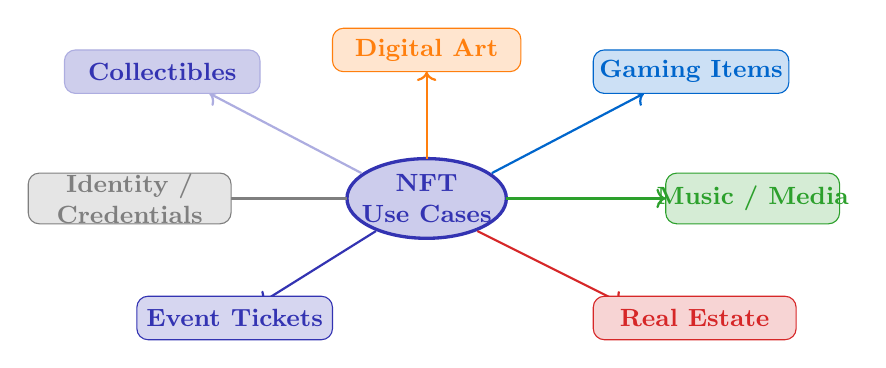
\begin{tikzpicture}[scale=0.92]
  % Center hub
  \draw[fill=mlpurple!25, draw=mlpurple, very thick] (5.5,2.75) ellipse (1.1 and 0.55);
  \node[font=\small\bfseries, mlpurple, align=center] at (5.5,2.75) {NFT\\Use Cases};

  % Spoke 1: Digital Art (top)
  \draw[->, thick, mlorange] (5.5,3.3) -- (5.5,4.5);
  \draw[fill=mlorange!20, draw=mlorange, rounded corners=4pt] (4.2,4.5) rectangle (6.8,5.1);
  \node[font=\small\bfseries, mlorange, align=center] at (5.5,4.8) {Digital Art};

  % Spoke 2: Gaming Items (top-right)
  \draw[->, thick, mlblue] (6.4,3.1) -- (8.5,4.2);
  \draw[fill=mlblue!20, draw=mlblue, rounded corners=4pt] (7.8,4.2) rectangle (10.5,4.8);
  \node[font=\small\bfseries, mlblue, align=center] at (9.15,4.5) {Gaming Items};

  % Spoke 3: Music / Media (right)
  \draw[->, thick, mlgreen] (6.6,2.75) -- (8.8,2.75);
  \draw[fill=mlgreen!20, draw=mlgreen, rounded corners=4pt] (8.8,2.4) rectangle (11.2,3.1);
  \node[font=\small\bfseries, mlgreen, align=center] at (10.0,2.75) {Music / Media};

  % Spoke 4: Real Estate (bottom-right)
  \draw[->, thick, mlred] (6.2,2.3) -- (8.2,1.3);
  \draw[fill=mlred!20, draw=mlred, rounded corners=4pt] (7.8,0.8) rectangle (10.6,1.4);
  \node[font=\small\bfseries, mlred, align=center] at (9.2,1.1) {Real Estate};

  % Spoke 5: Event Tickets (bottom-left)
  \draw[->, thick, mlpurple] (4.8,2.3) -- (3.2,1.3);
  \draw[fill=mlpurple!20, draw=mlpurple, rounded corners=4pt] (1.5,0.8) rectangle (4.2,1.4);
  \node[font=\small\bfseries, mlpurple, align=center] at (2.85,1.1) {Event Tickets};

  % Spoke 6: Identity / Credentials (left)
  \draw[->, thick, mlgray] (4.4,2.75) -- (2.2,2.75);
  \draw[fill=mlgray!20, draw=mlgray, rounded corners=4pt] (0.0,2.4) rectangle (2.8,3.1);
  \node[font=\small\bfseries, mlgray, align=center] at (1.4,2.75) {Identity /\\Credentials};

  % Spoke 7: top-left (Collectibles)
  \draw[->, thick, mllavender] (4.6,3.1) -- (2.5,4.2);
  \draw[fill=mllavender!60, draw=mllavender, rounded corners=4pt] (0.5,4.2) rectangle (3.2,4.8);
  \node[font=\small\bfseries, mlpurple, align=center] at (1.85,4.5) {Collectibles};
\end{tikzpicture}

\bottomnote{NFTs extend far beyond art -- they represent any unique digital or real-world asset.}
\end{frame}

% ==================== FRAME 8: NFTs BY THE NUMBERS ====================
\begin{frame}{NFTs by the Numbers}
\centering
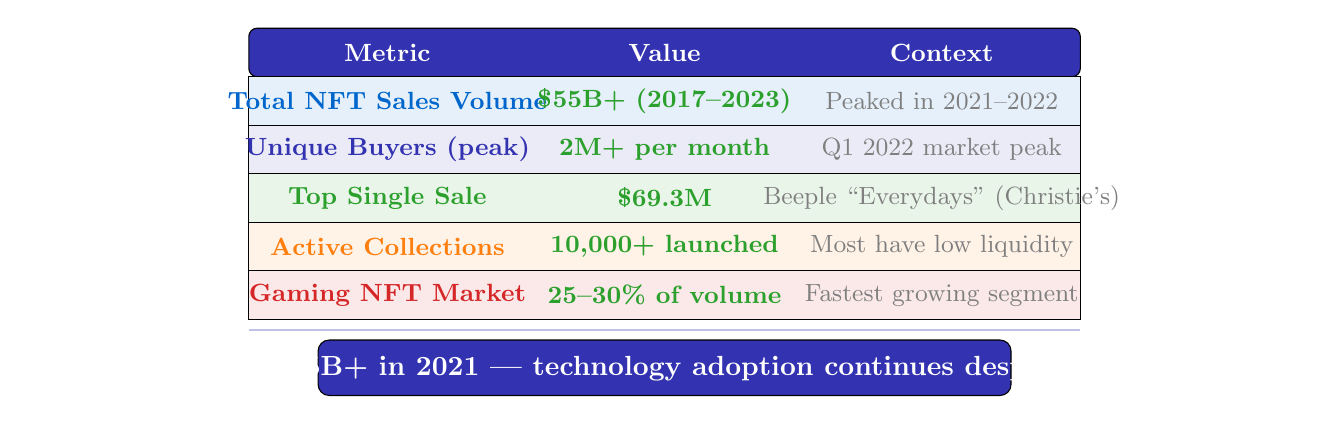
\begin{tikzpicture}[scale=0.88]
  % Table header
  \draw[fill=mlpurple, rounded corners=3pt] (0,5.2) rectangle (12,5.9);
  \node[font=\small\bfseries, white] at (2.0,5.55) {Metric};
  \node[font=\small\bfseries, white] at (6.0,5.55) {Value};
  \node[font=\small\bfseries, white] at (10.0,5.55) {Context};

  % Row 1
  \draw[fill=mlblue!10] (0,4.5) rectangle (12,5.2);
  \node[font=\small\bfseries, mlblue] at (2.0,4.85) {Total NFT Sales Volume};
  \node[font=\small\bfseries, mlgreen] at (6.0,4.85) {\$55B+ (2017--2023)};
  \node[font=\small, mlgray, align=center] at (10.0,4.85) {Peaked in 2021--2022};

  % Row 2
  \draw[fill=mlpurple!10] (0,3.8) rectangle (12,4.5);
  \node[font=\small\bfseries, mlpurple] at (2.0,4.15) {Unique Buyers (peak)};
  \node[font=\small\bfseries, mlgreen] at (6.0,4.15) {2M+ per month};
  \node[font=\small, mlgray, align=center] at (10.0,4.15) {Q1 2022 market peak};

  % Row 3
  \draw[fill=mlgreen!10] (0,3.1) rectangle (12,3.8);
  \node[font=\small\bfseries, mlgreen] at (2.0,3.45) {Top Single Sale};
  \node[font=\small\bfseries, mlgreen] at (6.0,3.45) {\$69.3M};
  \node[font=\small, mlgray, align=center] at (10.0,3.45) {Beeple ``Everydays'' (Christie's)};

  % Row 4
  \draw[fill=mlorange!10] (0,2.4) rectangle (12,3.1);
  \node[font=\small\bfseries, mlorange] at (2.0,2.75) {Active Collections};
  \node[font=\small\bfseries, mlgreen] at (6.0,2.75) {10,000+ launched};
  \node[font=\small, mlgray, align=center] at (10.0,2.75) {Most have low liquidity};

  % Row 5
  \draw[fill=mlred!10] (0,1.7) rectangle (12,2.4);
  \node[font=\small\bfseries, mlred] at (2.0,2.05) {Gaming NFT Market};
  \node[font=\small\bfseries, mlgreen] at (6.0,2.05) {25--30\% of volume};
  \node[font=\small, mlgray, align=center] at (10.0,2.05) {Fastest growing segment};

  % Divider
  \draw[mllavender2, thick] (0,1.55) -- (12,1.55);

  % Summary bar
  \draw[fill=mlpurple, rounded corners=4pt] (1.0,0.6) rectangle (11.0,1.4);
  \node[font=\normalsize\bfseries, white, align=center] at (6.0,1.0)
       {NFTs peaked at \$25B+ in 2021 --- technology adoption continues despite price correction};
\end{tikzpicture}

\bottomnote{Despite market cooling, NFT technology adoption continues in gaming, identity, and real-world assets.}
\end{frame}

% ==================== FRAME 9: THE RISKS OF NFTs ====================
\begin{frame}{The Risks of NFTs}
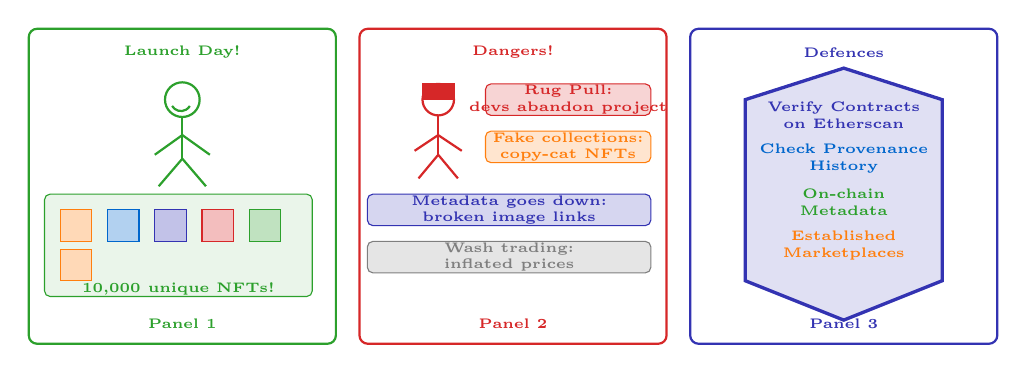
\begin{tikzpicture}
  % Panel borders
  \draw[thick, mlgreen,  rounded corners=3pt] (0.1,0.2) rectangle (4.0,4.2);
  \draw[thick, mlred,    rounded corners=3pt] (4.3,0.2) rectangle (8.2,4.2);
  \draw[thick, mlpurple, rounded corners=3pt] (8.5,0.2) rectangle (12.4,4.2);

  % --- Panel 1: Developer happy launching collection ---
  \node[font=\tiny\bfseries, mlgreen] at (2.05,3.9) {Launch Day!};
  % Developer stick figure (happy)
  \draw[mlgreen,thick] (2.05,3.3) circle (0.22);
  \draw[mlgreen,thick] (1.92,3.22) arc (210:330:0.13);
  \draw[mlgreen,thick] (2.05,3.08) -- (2.05,2.55);
  \draw[mlgreen,thick] (2.05,2.85) -- (1.7,2.6);
  \draw[mlgreen,thick] (2.05,2.85) -- (2.4,2.6);
  \draw[mlgreen,thick] (2.05,2.55) -- (1.75,2.2);
  \draw[mlgreen,thick] (2.05,2.55) -- (2.35,2.2);
  % NFT grid visual
  \draw[fill=mlgreen!10, draw=mlgreen, rounded corners=2pt] (0.3,0.8) rectangle (3.7,2.1);
  % 6 small NFT squares
  \draw[fill=mlorange!30, draw=mlorange] (0.5,1.5) rectangle (0.9,1.9);
  \draw[fill=mlblue!30, draw=mlblue]    (1.1,1.5) rectangle (1.5,1.9);
  \draw[fill=mlpurple!30, draw=mlpurple] (1.7,1.5) rectangle (2.1,1.9);
  \draw[fill=mlred!30, draw=mlred]      (2.3,1.5) rectangle (2.7,1.9);
  \draw[fill=mlgreen!30, draw=mlgreen]  (2.9,1.5) rectangle (3.3,1.9);
  \draw[fill=mlorange!30, draw=mlorange] (0.5,1.0) rectangle (0.9,1.4);
  \node[font=\tiny\bfseries, mlgreen, align=center] at (2.0,0.9) {10,000 unique NFTs!};
  \node[font=\tiny\bfseries, mlgreen] at (2.05,0.45) {Panel 1};

  % --- Panel 2: Red warnings ---
  \node[font=\tiny\bfseries, mlred] at (6.25,3.9) {Dangers!};
  % Hacker figure
  \draw[mlred,thick] (5.3,3.3) circle (0.20);
  \draw[fill=mlred!30, mlred] (5.1,3.3) rectangle (5.5,3.5);
  \node[font=\tiny, mlred] at (5.3,3.4) {hkr};
  \draw[mlred,thick] (5.3,3.1) -- (5.3,2.6);
  \draw[mlred,thick] (5.3,2.85) -- (5.0,2.65);
  \draw[mlred,thick] (5.3,2.85) -- (5.6,2.65);
  \draw[mlred,thick] (5.3,2.6)  -- (5.05,2.3);
  \draw[mlred,thick] (5.3,2.6)  -- (5.55,2.3);
  % Warning labels
  \draw[fill=mlred!20, draw=mlred, rounded corners=2pt] (5.9,3.1) rectangle (8.0,3.5);
  \node[font=\tiny\bfseries, mlred, align=center] at (6.95,3.3) {Rug Pull:\\devs abandon project};
  \draw[fill=mlorange!20, draw=mlorange, rounded corners=2pt] (5.9,2.5) rectangle (8.0,2.9);
  \node[font=\tiny\bfseries, mlorange, align=center] at (6.95,2.7) {Fake collections:\\copy-cat NFTs};
  \draw[fill=mlpurple!20, draw=mlpurple, rounded corners=2pt] (4.4,1.7) rectangle (8.0,2.1);
  \node[font=\tiny\bfseries, mlpurple, align=center] at (6.2,1.9) {Metadata goes down:\\broken image links};
  \draw[fill=mlgray!20, draw=mlgray, rounded corners=2pt] (4.4,1.1) rectangle (8.0,1.5);
  \node[font=\tiny\bfseries, mlgray, align=center] at (6.2,1.3) {Wash trading:\\inflated prices};
  \node[font=\tiny\bfseries, mlred] at (6.25,0.45) {Panel 2};

  % --- Panel 3: Defence shield ---
  \node[font=\tiny\bfseries, mlpurple] at (10.45,3.9) {Defences};
  % Shield shape
  \draw[fill=mlpurple!15, draw=mlpurple, very thick]
       (9.2,1.0) -- (9.2,3.3) -- (10.45,3.7) -- (11.7,3.3) -- (11.7,1.0) -- (10.45,0.5) -- cycle;
  % Defence items inside shield
  \node[font=\tiny\bfseries, mlpurple, align=center] at (10.45,3.1) {Verify Contracts\\on Etherscan};
  \node[font=\tiny\bfseries, mlblue, align=center]   at (10.45,2.55) {Check Provenance\\History};
  \node[font=\tiny\bfseries, mlgreen, align=center]  at (10.45,2.0) {On-chain\\Metadata};
  \node[font=\tiny\bfseries, mlorange, align=center] at (10.45,1.45) {Established\\Marketplaces};
  \node[font=\tiny\bfseries, mlpurple] at (10.45,0.45) {Panel 3};
\end{tikzpicture}

\bottomnote{NFT buyers face unique risks: rug pulls, counterfeit collections, and metadata permanence.}
\end{frame}

% ==================== FRAME 10: KEY TAKEAWAYS ====================
\begin{frame}{Key Takeaways}
\centering
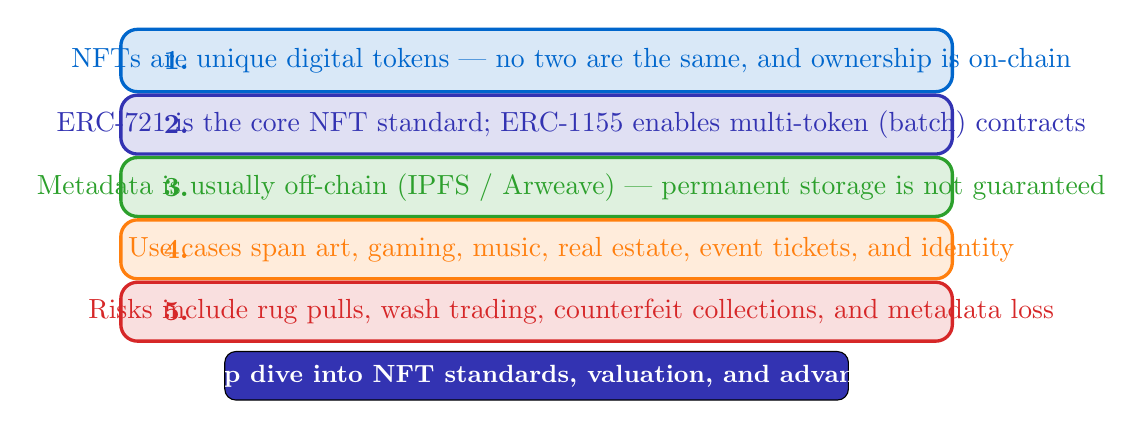
\begin{tikzpicture}[scale=0.88]
  % Box 1
  \draw[fill=mlblue!15, draw=mlblue, very thick, rounded corners=6pt]
       (0,4.5) rectangle (12,5.4);
  \node[font=\normalsize\bfseries, mlblue] at (0.8,4.95) {1.};
  \node[font=\normalsize, mlblue, align=left] at (6.5,4.95)
       {NFTs are unique digital tokens --- no two are the same, and ownership is on-chain};

  % Box 2
  \draw[fill=mlpurple!15, draw=mlpurple, very thick, rounded corners=6pt]
       (0,3.6) rectangle (12,4.45);
  \node[font=\normalsize\bfseries, mlpurple] at (0.8,4.02) {2.};
  \node[font=\normalsize, mlpurple, align=left] at (6.5,4.02)
       {ERC-721 is the core NFT standard; ERC-1155 enables multi-token (batch) contracts};

  % Box 3
  \draw[fill=mlgreen!15, draw=mlgreen, very thick, rounded corners=6pt]
       (0,2.7) rectangle (12,3.55);
  \node[font=\normalsize\bfseries, mlgreen] at (0.8,3.12) {3.};
  \node[font=\normalsize, mlgreen, align=left] at (6.5,3.12)
       {Metadata is usually off-chain (IPFS / Arweave) --- permanent storage is not guaranteed};

  % Box 4
  \draw[fill=mlorange!15, draw=mlorange, very thick, rounded corners=6pt]
       (0,1.8) rectangle (12,2.65);
  \node[font=\normalsize\bfseries, mlorange] at (0.8,2.22) {4.};
  \node[font=\normalsize, mlorange, align=left] at (6.5,2.22)
       {Use cases span art, gaming, music, real estate, event tickets, and identity};

  % Box 5
  \draw[fill=mlred!15, draw=mlred, very thick, rounded corners=6pt]
       (0,0.9) rectangle (12,1.75);
  \node[font=\normalsize\bfseries, mlred] at (0.8,1.32) {5.};
  \node[font=\normalsize, mlred, align=left] at (6.5,1.32)
       {Risks include rug pulls, wash trading, counterfeit collections, and metadata loss};

  % Teaser
  \draw[fill=mlpurple, rounded corners=4pt] (1.5,0.05) rectangle (10.5,0.75);
  \node[font=\small\bfseries, white, align=center] at (6.0,0.40)
       {Next: Deep dive into NFT standards, valuation, and advanced topics};
\end{tikzpicture}

\bottomnote{Next: Deep dive into NFT standards, valuation, and advanced topics.}
\end{frame}

\end{document}
